
% This LaTeX was auto-generated from MATLAB code.
% To make changes, update the MATLAB code and republish this document.

\documentclass{article}
\usepackage{graphicx}
\usepackage{color}

\sloppy
\definecolor{lightgray}{gray}{0.5}
\setlength{\parindent}{0pt}

\begin{document}

    
    \begin{verbatim}
R = 20;
L = 10;
C = 1;

den = [R*L*C, L, R];

G11 = tf([R*C, 1],den);
G12 = tf([1],den);
G21 = G12;
G22 = tf([L*C, 0, 1],den);

sys = [G11, G12; G21, G22]

sys.InputName = ['V_1'; 'V_2'];
sys.OutputName = ['I_1'; 'I_2'];

bode(sys)
grid on
\end{verbatim}

        \color{lightgray} \begin{verbatim}
sys =
 
  From input 1 to output...
            20 s + 1
   1:  -------------------
       200 s^2 + 10 s + 20
 
                1
   2:  -------------------
       200 s^2 + 10 s + 20
 
  From input 2 to output...
                1
   1:  -------------------
       200 s^2 + 10 s + 20
 
           10 s^2 + 1
   2:  -------------------
       200 s^2 + 10 s + 20
 
Continuous-time transfer function.

\end{verbatim} \color{black}
 
\centering   
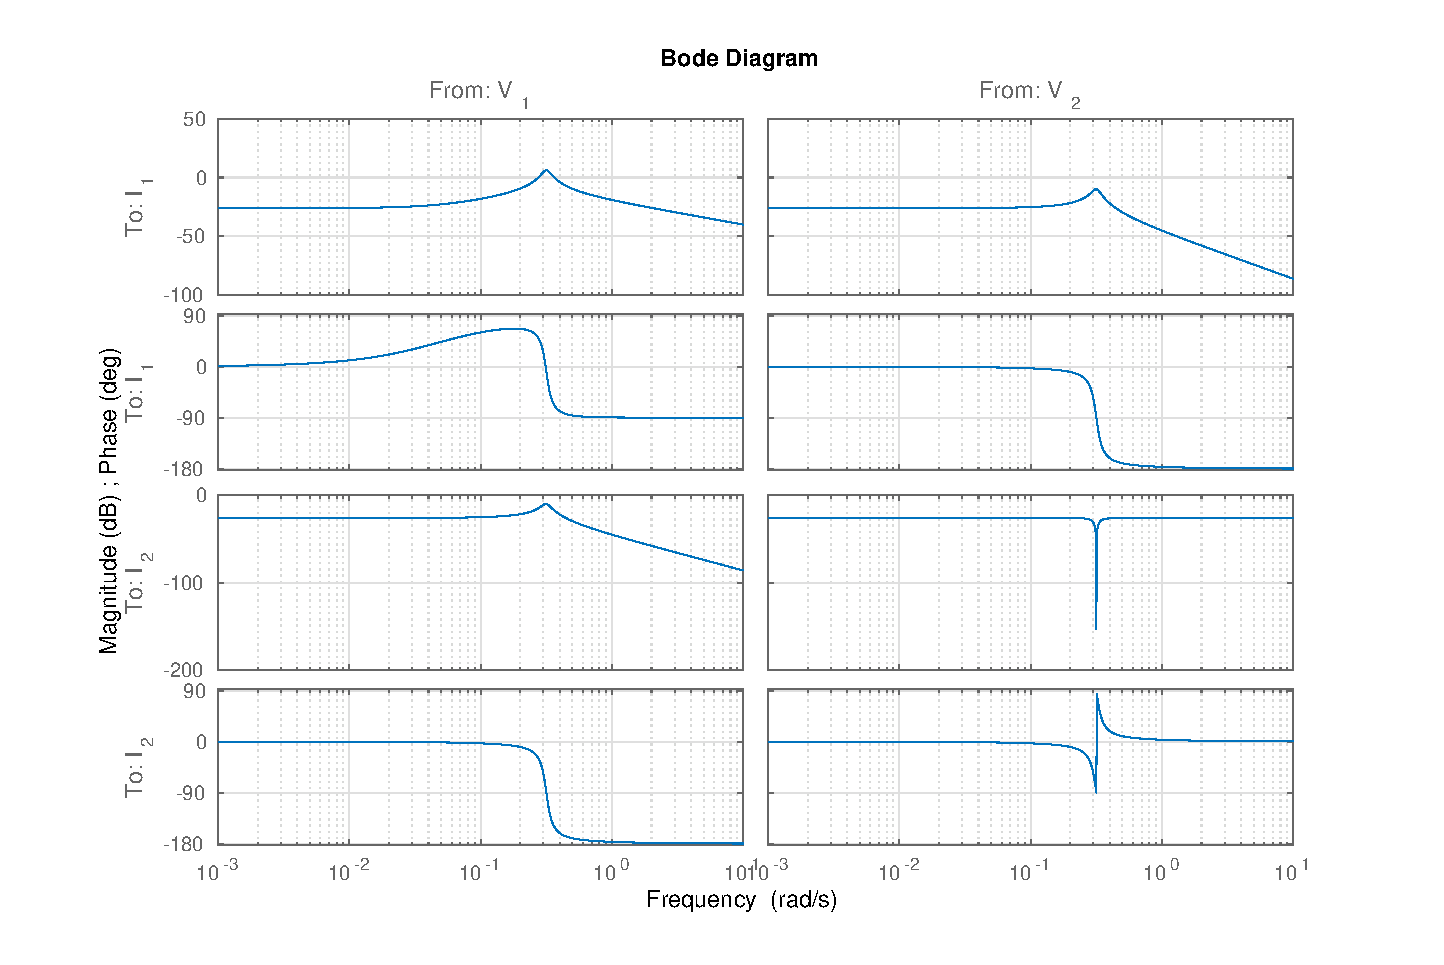
\includegraphics [width=5in]{Q9_11_01.eps}



\end{document}
    
